\section{Introdu��o}

\begin{frame}\frametitle{Introdu��o}
\begin{itemize}
	\item Um problema t�pico na visualiza��o de modelos 3D � que as caracter�sticas (\emph{features}) mais interessantes podem estar obstru�das por outras partes menos importentes.
	\item Ilustra��es t�cnicas e m�dicas resolvem este problema alterando o n�vel de abstra��o visual ou alterando a disposi��o espacial:
	\begin{columns}[T]
	\begin{column}{5cm}
	\begin{itemize}
		\item \alert<1,5>{Cut-away view}
		\item \alert<2,5>{Ghosted view}
		\item \alert<3,5>{Section view}
		\item \alert<4,5>{Exploded view}
	\end{itemize}
	\vspace{3cm} 
	\end{column}
	\begin{column}{5cm}
	\begin{overprint}
		\includegraphics<1>[height=100.0px]{img/IllustrativeVisualization1}
		\includegraphics<2>[height=100.0px]{img/IllustrativeVisualization2}
		\includegraphics<3>[height=100.0px]{img/IllustrativeVisualization3}
		\includegraphics<4>[height=100.0px]{img/IllustrativeVisualization4}
	\end{overprint}
	\only<5>{Smart Visibility Techniques \cite{Viola-05-Smart}}
	\end{column}
	\end{columns}
\end{itemize}
\end{frame}

\begin{frame}\frametitle{\emph{Smart visibility}}
\begin{itemize}
	\item Uma "visibilidade inteligente" leva em considera��o:
	\begin{itemize}
		\item A \textbf{relev�ncia dos objetos e suas caracter�sticas}, e n�o apenas o seu posicionamento no espa�o. Um objeto importante pode ser visualizado apesar de estar sendo obstru�do por algum outro objeto mais pr�ximo do observador.
		\item A \textbf{familiaridade do observador com os objetos}. A partir de um objeto parcialmente vis�vel, o observador pode complet�-lo mentalmente, com base em sua experi�ncia.
	\end{itemize}
\end{itemize}
\end{frame}

\begin{frame}\frametitle{Vistas explodidas}
\begin{itemize}
	\item Vistas explodidas modificam o posicionamento espacial dos componentes de um objeto para que os mais "interessantes" estejam vis�veis.
	\item Permitem o entendimento da estrutura global do objeto e a rela��o espacial entre os componentes.
\end{itemize}
\begin{center}
	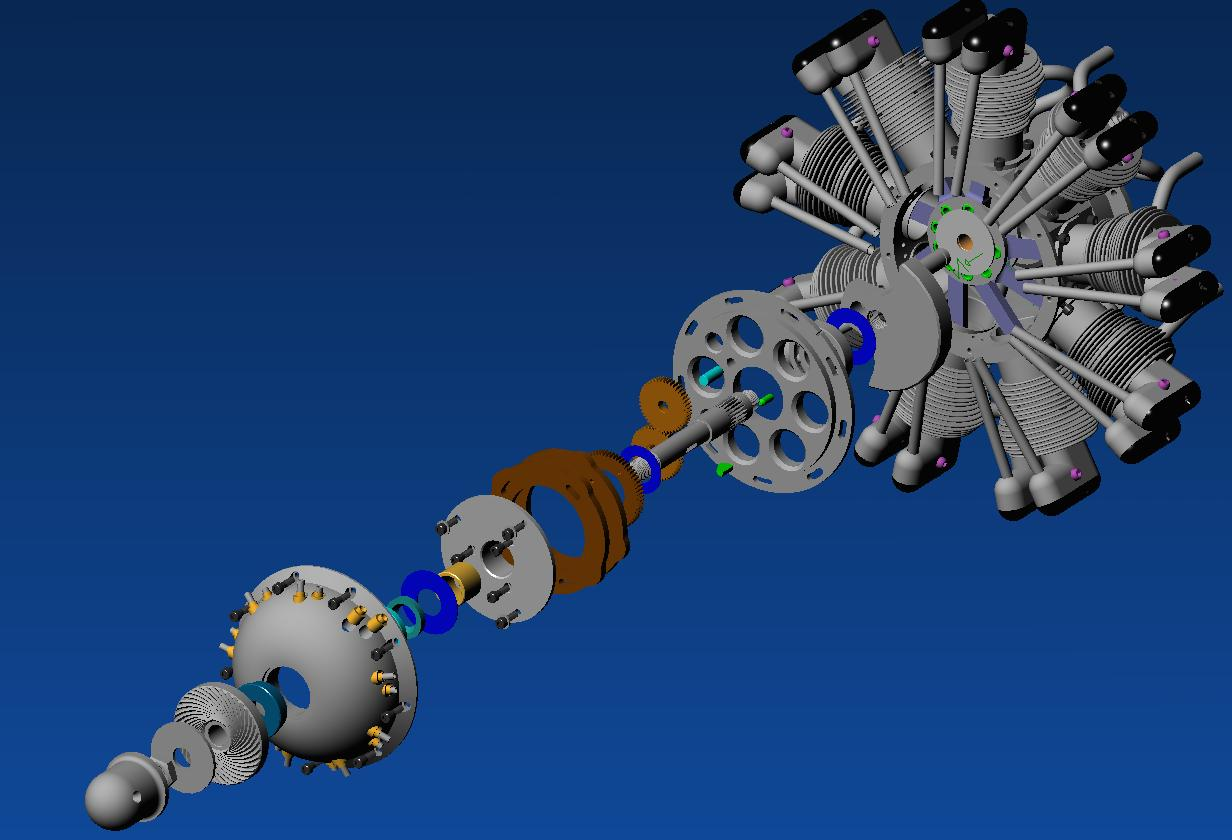
\includegraphics[height=100.0px]{img/engine}
\end{center}	
\end{frame}


%Definir vista explodida de acordo com o artigo 1
%Falar do artigo 2 e situar a vista explodida em rela��o a outras visualiza��es inteligentes
%Criar se��o "Trabalhos relacionados a vista explodida"


